\documentclass[12pt, twoside]{article}
\usepackage[letterpaper, margin=1in, headsep=0.5in]{geometry}
\usepackage[english]{babel}
\usepackage[utf8]{inputenc}
\usepackage{amsmath}
\usepackage{amsfonts}
\usepackage{amssymb}
\usepackage{tikz}
\usetikzlibrary{quotes, angles}
\usepackage{venndiagram}
\usepackage{multicol}

\usepackage{pgfplots}
\pgfplotsset{width=10cm,compat=1.9}
\usepgfplotslibrary{statistics}
\usepackage{pgfplotstable}


\usepackage{fancyhdr}
\pagestyle{fancy}
\fancyhf{}
\renewcommand{\headrulewidth}{0pt} % disable the underline of the header
%\renewcommand{\baselinestretch}{1.5}

\fancyhead[RE]{\thepage}
\fancyhead[RO]{\thepage \\ Name: \hspace{3cm}}
\fancyhead[L]{BECA / Dr. Huson / IB Math\\* 20 November 2019}


\begin{document}
\subsubsection*{2.16 Do Now: Linear regression and correlation}
\begin{enumerate}
 
  \item The flash rate of fireflies depends on various factors, including temperature. As the temperature drops, the flash rate slows down.
  
  
  %\begin{enumerate}
  
  %\item  Assume the given data
  
  %\subsubsection*{Table of timing data}
  
  Firefly field data (simulated) where $T$ is the temperature and $f(T)$ is the number of seconds between flashes. \\[10pt]
  \begin{tabular}{|c|r|r|r|r|r|}
  \hline
  $T$ & 54 & 60 & 64 & 70 & 75 \\ [3pt]
  \hline
  $f(T)$ & 5 & 8 & 10 & 11 & 13  \\  [3pt]
  \hline
  \end{tabular}
  \begin{enumerate}
      \item Plot the data in the table on the grid below \\
      (one point is plotted for you)
      \item Calculate $\bar{x}$ and $\bar{y}$
      \item Enter the data in your calculator
  \end{enumerate}
  
  \vspace{1in}
  %\item
  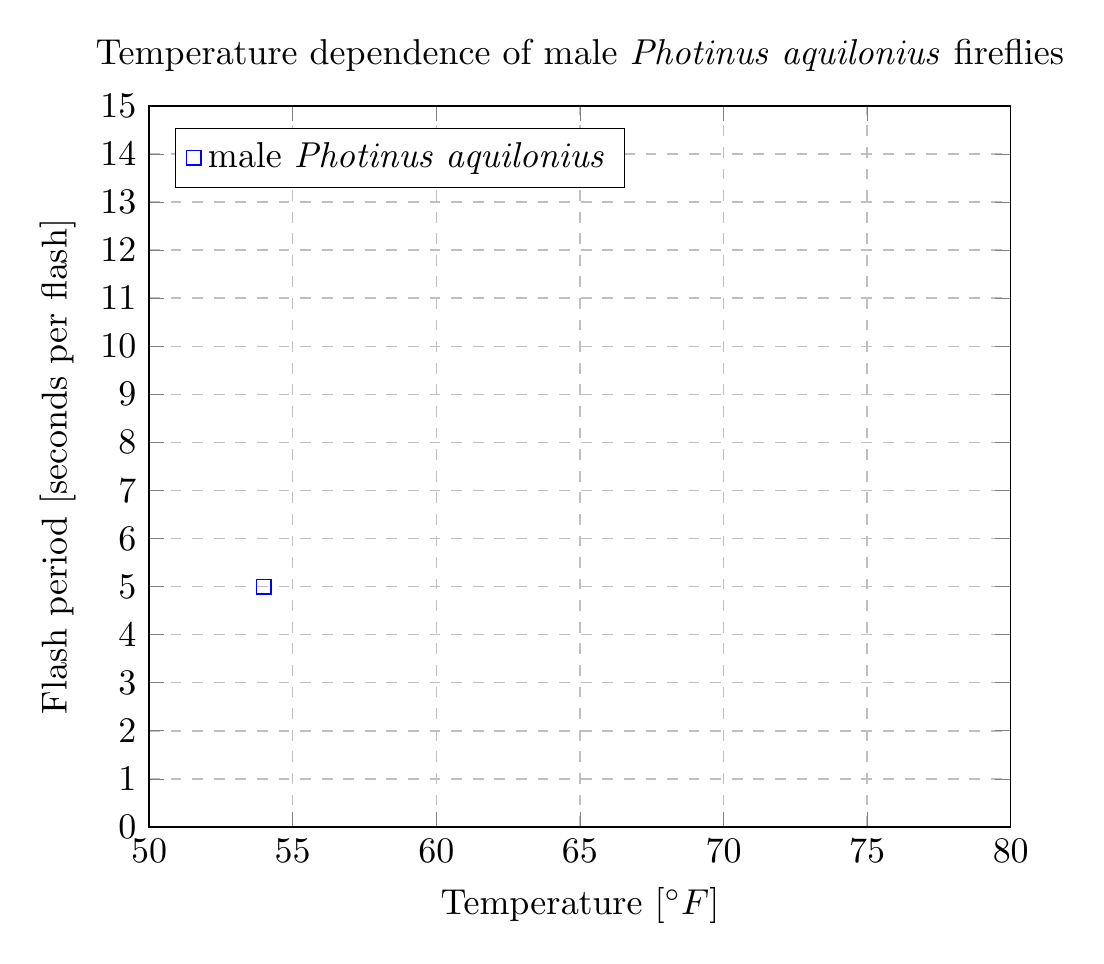
\begin{tikzpicture}[scale=1.3]
  \begin{axis}[
      title={Temperature dependence of male \emph{Photinus aquilonius} fireflies},
      xlabel={Temperature [$^{\circ}F$]},
      ylabel={Flash period [seconds per flash]},
      xmin=50, xmax=80,
      ymin=0, ymax=15,
      xtick={50,55,60,65,70,75,80},
      ytick={0,1,2,3,4,5,6,7,8,9,10,11,12,13,14,15},
      legend pos=north west,
      xmajorgrids=true,
      ymajorgrids=true,
      grid style=dashed,
  ]
  \addplot[only marks,
      color=blue,
      mark=square,
      ]
      coordinates {
      (54,5)%(60,8)(64,10)(70,11)(75,13)
      };
      \legend{male \emph{Photinus aquilonius}}
  \end{axis}
  \end{tikzpicture}
  
\newpage
\item Dr. Huson buys a new plant and measures how tall it is after a number of weeks. Some of his measurements are shown below. Plot the points in the grid below.
  \renewcommand{\arraystretch}{1.6}
    \begin{center}
      \begin{tabular}{|l|r|r|r|r|}
      \hline
      Weeks & 2 & 5 & 7 & 10\\
      \hline
      Height (cm) & 5 & 6 & 8 & 9 \\
      \hline
      \end{tabular}
    \end{center}

\begin{center} %4 quadrant regents grid w T-Chart
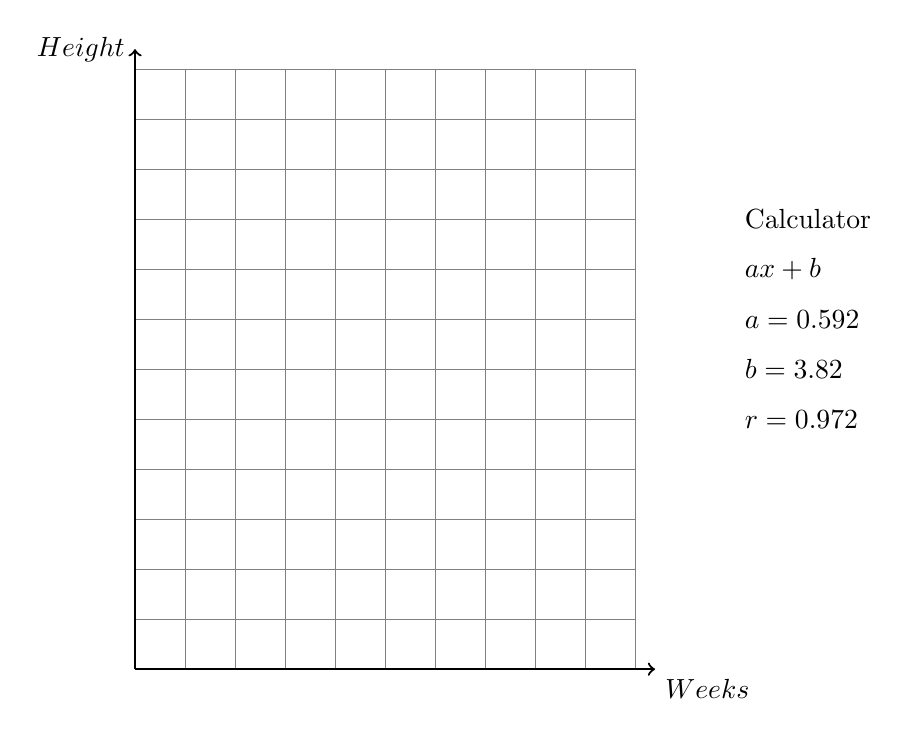
\begin{tikzpicture}[scale=.635]
  \draw [help lines] (0,0) grid (10,12);
  \draw [thick, ->] (0,0) -- (10.4,0) node [below right] {$Weeks$};
  \draw [thick, ->] (0,0)--(0,12.4) node [left] {$Height$};
  \node at (12,9)[right]{Calculator};
  \node at (12,8)[right]{$ax+b$};
  \node at (12,7)[right]{$a=0.592$};
  \node at (12,6)[right]{$b=3.82$};
  \node at (12,5)[right]{$r=0.972$};
\end{tikzpicture}
\end{center}
State, to the \emph{nearest tenth}, the linear regression equation that approximates the height, $y$, of the plants after $x$ weeks.\\[2cm]
Explain what the $y$-intercept means in the context of the problem. \\[3cm]
Explain what the slope means in the context of the problem.


\end{enumerate}
\end{document}
